\documentclass[
	classe=$2^{de}$,
	headerTitle=Activité
]{exercice}

\usetikzlibrary{calc}

\title{Activité : translation de figures}

\begin{document}

\maketitle

\begin{exercice}\
	\begin{center}
		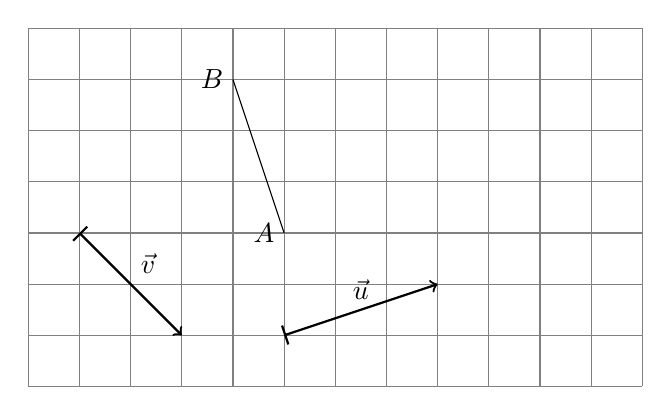
\begin{tikzpicture}[scale=0.65]
			\draw[thin,gray] (-5,-3) grid (7,4);
			\coordinate (A) at (0,0);
			\coordinate (B) at (-1,3);
			\coordinate (VecU) at (3,1);
			\coordinate (VecV) at (2,-2);

			\foreach \p in {A,B} {
					\node[left] at (\p) {$\p$};
				}
			\draw (A) -- (B);
			\draw[thick,|->] (0,-2) -- node[above] {$\vec{u}$} ++(VecU);
			\draw[thick,|->] (-4,0) -- node[above right] {$\vec{v}$} ++(VecV);

			\ifdefined\makeCorrection
				\draw[red] ($(A) + (VecU)$) node[left] {$A'$} -- ($(B) + (VecU)$) node[left] {$B'$};
				\draw[red] ($(A) + (VecU) + (VecV)$) node[left] {$A''$} -- ($(B) + (VecU) + (VecV)$) node[left] {$B''$};
			\fi
		\end{tikzpicture}
	\end{center}

	Sur la figure ci-dessus :
	\begin{enumerate}
		\item Placer le point $A'$, obtenu en translatant $A$ par le vecteur $\vec{u}$.
		\item Placer le point $B'$, obtenu en translatant $B$ par le vecteur $\vec{u}$. \medskip

		      Le segment $[A'B']$ est alors le translaté du segment $[AB]$ par le vecteur $\vec{u}$.
		\item Que remarque-t'on sur la figure $ABB'A'$ ? \correction{C'est un parallélogramme}.
		\item Construire $[A''B'']$ le translaté du segment $[AB]$ par $\vec{u} + \vec{v}$.
	\end{enumerate}
\end{exercice}

\begin{exercice}\
	\begin{center}
		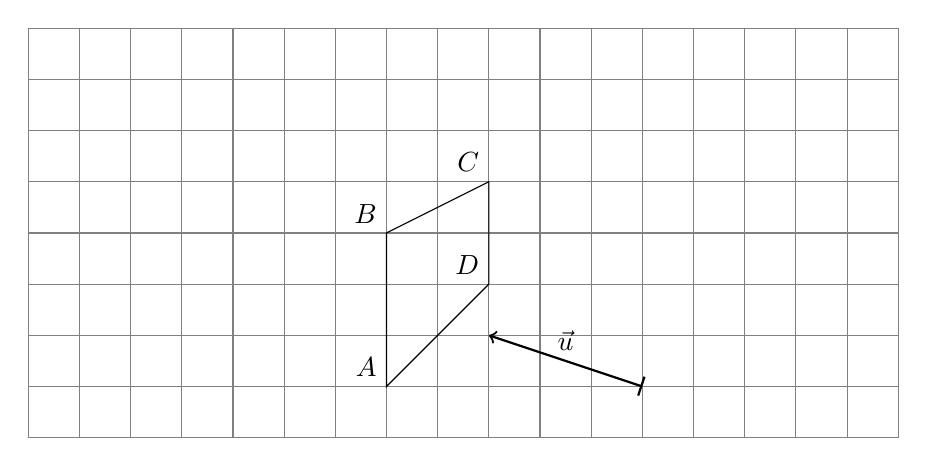
\begin{tikzpicture}[scale=0.65]
			\draw[thin,gray] (-7,-1) grid (10,7);
			\coordinate (A) at (0,0);
			\coordinate (B) at (0,3);
			\coordinate (C) at (2,4);
			\coordinate (D) at (2,2);

			\coordinate (VecBC) at ($(C) - (B)$);
			\coordinate (VecU) at (-3,1);

			\foreach \p in {A,B,C,D} {
					\node[above left] at (\p) {$\p$};
				}
			\draw (A) -- (B) -- (C) -- (D) -- cycle;
			\draw[thick,|->] (5,0) -- node[above] {$\vec{u}$} ++(VecU);

			\ifdefined\makeCorrection
				\draw[red] ($(A) + (VecU)$) -- ($(B) + (VecU)$) -- ($(C) + (VecU)$) -- ($(D) + (VecU)$) -- cycle;
				\draw[red] ($(A) + 2*(VecBC)$) -- ($(B) + 2*(VecBC)$) -- ($(C) + 2*(VecBC)$) -- ($(D) + 2*(VecBC)$) -- cycle;
			\fi
		\end{tikzpicture}
	\end{center}

	\begin{enumerate}
		\item Construire le translaté de la figure ABCDE par le vecteur $\vec{u}$.
		\item Construire le translaté de la figure ABCDE par le vecteur $2\vec{BC}$.
	\end{enumerate}
\end{exercice}

\begin{exercice}\
	\begin{center}
		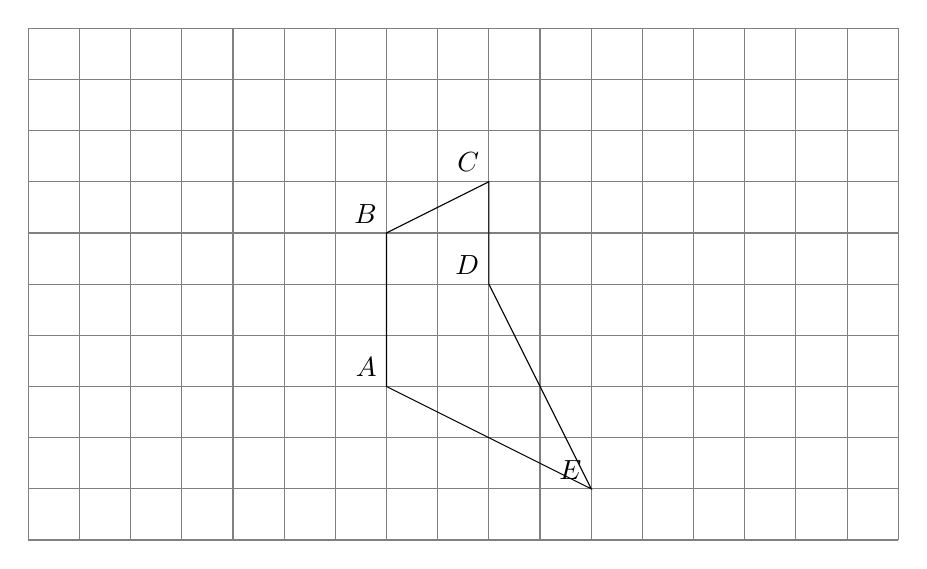
\begin{tikzpicture}[scale=0.65]
			\draw[thin,gray] (-7,-3) grid (10,7);
			\coordinate (A) at (0,0);
			\coordinate (B) at (0,3);
			\coordinate (C) at (2,4);
			\coordinate (D) at (2,2);
			\coordinate (E) at (4,-2);

			\coordinate (Vec1) at ($(D) + (C) - 2*(B)$);
			\coordinate (Vec2) at ($1.5*(A) - 1.5*(E) - 1/3*(B) + 1/3*(A)$);

			\foreach \p in {A,B,C,D,E} {
					\node[above left] at (\p) {$\p$};
				}
			\draw (A) -- (B) -- (C) -- (D) -- (E) -- cycle;

			\ifdefined\makeCorrection
				\draw[red] ($(A) + (Vec1)$) -- ($(B) + (Vec1)$) -- ($(C) + (Vec1)$) -- ($(D) + (Vec1)$) -- ($(E) + (Vec1)$) -- cycle;
				\draw[red] ($(A) + (Vec2)$) -- ($(B) + (Vec2)$) -- ($(C) + (Vec2)$) -- ($(D) + (Vec2)$) -- ($(E) + (Vec2)$) -- cycle;
			\fi
		\end{tikzpicture}
	\end{center}

	\begin{enumerate}
		\item Construire le translaté de la figure ABCDE par le vecteur $\vec{BD} + \vec{BC}$.
		\item Construire le translaté de la figure ABCDE par le vecteur $\frac{3}{2}\vec{EA} - \frac{1}{3}\vec{AB}$.
	\end{enumerate}
\end{exercice}

\end{document}